%% -*- coding: utf-8; -*-

% Use 'digital' option to enable back references. This option is recommended for digital pdf version
%\documentclass[phd,american,digital]{thesispuc}%english thesis
%\documentclass[mscr,american]{thesispuc}%english dissertation
%\documentclass[phd,brazilian]{thesispuc}%tese em portugês
\documentclass[msc,brazilian]{thesispuc}%disseretação em portuguŝ


%%%
%%% Additional Packages
%%%
\usepackage{tabularx}
\usepackage{multirow}
\usepackage{multicol}
\usepackage{colortbl}
\usepackage[%
    dvipsnames,
    svgnames,
    x11names,
    fixpdftex,
    table
]{xcolor}
\usepackage{numprint}
\usepackage{textcomp}
\usepackage{booktabs}
\usepackage{amsmath}
\usepackage{enumitem}
\usepackage{amssymb}
% ABNT reference style package. The current style is the alphabetical order, if you need
% change to citation order, change in the line above 'alf' to 'num', also at the end replace
% bibliographystyle with the commented version.
\usepackage[num]{abntex2cite}
%\usepackage{tikz}
%\usepackage[linesnumbered, ruled, vlined]{algorithm2e}
%\usepackage{pgfplots,pgfplotstable} 
%\usepackage{array}


%% numprint 
\npthousandsep{.}
\npdecimalsign{,}

%% ThesisPUC option
%\tablesmode{fig} %% [nada, fig, tab ou figtab]
%\algoritmsmode{none} %% [none ou use] %% Default is [use]
%\codesmode{none} %% [none ou use] %% Default is [use]
%\abreviationsmode{none} %% [none ou use] %% Default is [use]

\tablesmode{figtab}

\algorithmsmode{none}
\codesmode{use}
\abreviationsmode{none}

% \makeatletter  \renewcommand\@biblabel[1]{#1}  \makeatother

%%%
%%% Counters
%%%

%% uncomment and change for other depth values
\setcounter{tocdepth}{1}
%\setcounter{lofdepth}{3}
%\setcounter{lotdepth}{3}
%\setcounter{secnumdepth}{3}

%%%
%%% Misc.
%%%

\usecolour{true}
%% \graphicspath{ {./figuras/} }
%% https://www.overleaf.com/learn/latex/Inserting_Images
\citebrackets[]

\renewcommand{\arraystretch}{1.5}


%%%
%%% Titulos
%%%

\autor{Antenor Moreira de Barros Leal}
\autorR{Leal, Antenor Moreira de Barros}

\advisor{Adriano Francisco Branco}{Prof.}
\advisorR{Branco, Adriano Francisco}
% If the advisor's department is different from author's department, uncomment the next line and type the correct name and acronym of advisor's institution.
%\advisorInst{institution name}{acronym}

%\coadvisor{Otávio da Fonseca Martins Gomes}{Dr.}
%\coadvisorR{da Fonseca Martins Gomes, Otávio}
%\coadvisorInst{Centro de Tecnologia Mineral}{CETEM/MCTI}

\title{Aplicativo web de auxílio a navegação aérea}
\titleuk{Aerial navigation aid web application}

%%\subtitulo{Aqui vai o subtitulo caso precise}

\day{16}
\month{Abril}
\year{2024}

\city{Rio de Janeiro}
\CDD{004} 
\department{Informática}
\program{\mbox{Engenharia} da \mbox{Computação}}
\school{\mbox{Engenharia} da \mbox{Computação}}
\university{Pontifícia Universidade Católica do Rio de Janeiro}
\uni{PUC-Rio}


%%%
%%% Jury
%%%

\jury{%
  \jurymember{xxxxxxxxxxxxxxxx}{Prof.}
    {Departamento de Informática}{PUC-Rio}
  \jurymember{xxxxxxxxxxxxxxx}{Prof.}
    {Departamento de Informática}{PUC-Rio}
   \jurymember{xxxxxxxxxxxxxxx}{Prof.}
    {Departamento de Informática}{PUC-Rio}
}


%%%
%%% Personal Resume
%%%

\resume{%
% If it fit in one line use this command:
\makebox[\textwidth][s]{Graduando em Engenharia da Computação na PUC - Rio}%
% If not just type your resume without any special command 
}


%%%
%%% Catalog prekeywords
%%%

\catalogprekeywords{%
  \catalogprekey{Informática}%
}

%%%
%%% Keywords - Don't use % at the end of /key dfinition
%%%

\keywords{%
    \key{Aviação}
    \key{Navegação}
    \key{Aplicativo}
    \key{Algoritmo}
}

\keywordsuk{%
    \key{Aviation}
    \key{Navigation}
    \key{Application}
    \key{Algoritm}
}


%%%
%%% Abstract
%%%

\abstract{%
Trata-se de um aplicativo web de código aberto para auxiliar usuários de simuladores de voo que não possuem
acesso à ferramenta (Electronic Flight Bag) que um piloto de linha aérea teria. Ao entrar no aplicativo, o usuário
se depara com a lista de aeroportos cadastrados e, ao escolher um, são exibidas informações da pista,
frequências do aeroporto (torre, solo, ATIS, etc.), e frequências de navegação (ILS, VOR, etc.). Também são
apresentadas as informações das condições meteorológicas atuais do aeródromo (vento, visibilidade,
temperatura, etc.), tanto no formato oficial (METAR), obtidas a cada hora de uma API externa, como em um texto
em linguagem natural para melhor entendimento do jogador iniciante. Um usuário com permissão de
administrador pode adicionar e editar aeroportos. A partir de informação do vento, a pista em uso é calculada.
} 

\abstractuk{%
xxxxxx
}


%%%
%%% Dedication
%%%

\dedication{%
  xxxxxxxxxxxxxxxxxxxxxxxxxxxxxxxx
}

%%%
%%% Epigraph
%%%

\epigraph{%
}
\epigraphauthor{xxxxxxxxxxxxxxxx}
\epigraphbook{xxxxxxxxxxxxxxxxxxepígrafex}


\begin{document}
  \chapter{Decodificação do METAR}

\section{Introdução}
O metar é um protocolo de transmissão de dados meteorologicos atuais de um aeroporto ou aeródromo.
O metar é formado por itens separados por espaço. Cada item correponde a uma
unidade mínima de informação meteorológica. Com os dados de sensores instalados no aeródromo, a
cada hora é publicado um novo METAR que é válido aquela hora. Em casos excepcionais quando o as condições de tempo 
estiverem mudando repentinamente um METAR pode ser atualizado a cada meia hora. \cite{metar-speci}

\section{Exemplo}
O METAR no aeroporto de Fortaleza \cite{metar-sbfz}, no dia 17 de abril de 2024 as 10:54 foi
\begin{verbatim}
    171300Z 15010KT 9999 BKN019 SCT025 FEW030TCU BKN100 30/25 Q1011
\end{verbatim}

"SBFZ" se refere ao código ICAO (International Civil Aviation Organization  do aeroporto, não
confudir com o código IATA (International Air Transport Association) que é formado por três letras.
O aeroporto Pinto Martins possui o código IATA FOR, o público geral parece conhecer mais este código, mas na aviação
costuma-se usar mais o código ICAO, pois \textit{todos} os aeródromos possuem um, enquanto o IATA só 
é presente em aeroportos onde há processamento de bagagem \cite{iata-codes} \cite{icao-codes}. 

O ICAO é formado por quatro letras em que a primeira é o prefixo da região.
A América do Sul possui o prefixo "S",
o Brasil possui o prefixo "SB", por isso que o Aeroporto do Galeão, Guarulhos e Fortaleza possuem 
os códigos SBGL, SBGR e SBFZ, respecitvamente. Países com muitos aeroportos como os EUA, possuem
como prefixo a letra K, logo as três letras ficam livres, podendo assim terem mais códigos para uso.

\texttt{171300Z} significa que este METAR se refere ao dia 17 as 13 horas e zero minuto zulu. Horário
zulu é simplemente no fuso horário da longitude de zero grau e um minuto, chamado de hora UTC ou 
Coordinated Universal Time. \cite{UTC} Para que não haja confusões com os horários, a aviação internacionalmente
usa o horário UTC. Este METAR, será válido até as 13:59,
quando será substituído pelo metar iniciando com "SBRJ 171400Z".

Note que a seguinte expressão regular com três grupos de captura conseguem extrair o dia a hora e o minuto.

\begin{verbatim}
([0-9]{2})([0-9]{2})([0-9]{2})Z
\end{verbatim}

Em nossos explos os grupos serão: 

\begin{itemize}
  \item Grupo 1: 17
  \item Grupo 2: 14
  \item Grupo 3: 00
\end{itemize}

\texttt{15010KT} se refere a velocidade e direção do vento, os três primeiros algarismos a direção, em graus,
de onde o vento sopra e os últimos dois algarismos do módulo da velocidade do vento em nós (milhas
náuticas por hora). Neste caso o vento vem da direção 150 graus com velocidade de dez nós.
Com a expressão abaixo estraímos estas informações.

\begin{verbatim}
([0-9]{3})([0-9]{2})KT
\end{verbatim}

Existe também a notação com a letra G e a letra V. \texttt{10016G21KT 080V120} significa que há rajadas de
até 21kt e a direção do vento pode variar de 80 à 120 graus. Existem outros aeroportos que podem usar 
outras unidades para a velocidade do vento, mas no Brasil só é usado nós (kt).

\texttt{9999} Significa visibilidade ilimitada (maior ou igual a 10km). Se fosse 6000 a visibilidade 
seria de 6km.

\texttt{30/25} Temperatura 30°C e ponto de orvalho 25°C. Caso a temperatura seja negativa a letra M é adicionada
antes do número. M2/M5 significa temperatura -2°C e ponto de orvalho -5°C. \cite{metar-help}

\texttt{Q1012} O altímetro do avião deve ser referenciado para 1012 hecto pascal. Também pode ser usada
a unidade polegadas de mercúrio (mmHg), mas no Brasil esta não é usada no METAR.

\texttt{SCT025} Nuvens espalhadas (3/8 a 4/8 do céu com nuvens) em 2500 pés de altitude. 025 se refere ao
nível de voo (Flight Level) que é a altitude acima do nível médio do mar com divisão exata por 100.

\texttt{FEW030TCU} Poucas nuvens (1/8 a 2/8 do céu com nuvens) em 3000 pés de altitude. O sufixo TCU siginica que
há nuvens convectivas significativas. \cite {decea-mil}

\texttt{BKN100} Nuvens broken (5/8 a 7/8 do céu com nuvens) em 10000 pés de altitude.

Existe também o tipo OVC (overcast) que se refere a totalmente encoberto.

O objetivo do módulo de decoder é dar uma explicação semelhante a esta para qualquer tipo de METAR
de aeroportos no Brasil. O módulo usa várias expressões regulares para decodificar uma grande quantidade de informações,
porém não é exaustivo, foi dada a preferência a fenômenos que podem ocorrer no Brasil. Tirando o ICAO e a informação
do dia e hora, os itens de informação não possuem uma ordem fixa por isto o algorítmo, para cada item
precisa testar cada expressão regular até que haja o match. Caso algum item não corresponda e nehuma
expressão regular, este é descartado.

  \chapter{Modelo de Dados}

O modelo de dados foi feito para ser o mais simples possível para que futuras alterações
possam ser feitas facilmente. Abaixo está o diagrama entidade-relacionamento no qual
o nome no topo do retângulo identifica o nome da tabela. A lista abaixo mostra
as colunas dessas tabelas, com um ícone de uma chave preta para a \textit{chave primária} e 
uma chave verde para a \textit{chave estrangeira}.

Uma relação é denotada pelas setas ligando duas tabelas. A cardinalidade da relação é indicada
pelos números entre parênteses. 

Para a relação \texttt{Aerodrome-ILS}, temos (1, 1) para (0, n), significando que um aeródromo pode
ter zero ou mais frequências de ILS e esta só pode ser de um único aeródromo.

Já na relação \texttt{Aerodrome} com \texttt{Runway}, um aeródromo deve ter \texttt{uma ou mais} pistas.


\begin{figure}[ht]
    \begin{center}
    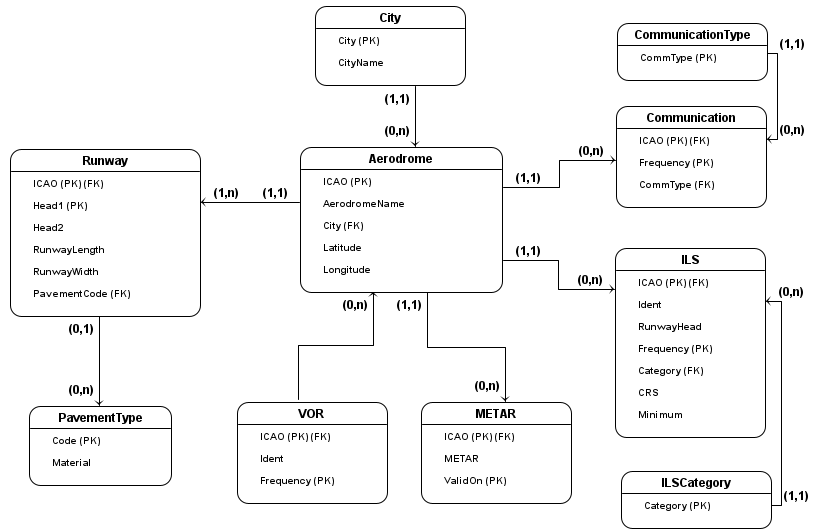
\includegraphics[width=400pt]{img/ERAero.png}
    \caption{Diagrama E/R}
    \label{fig:diagrama-er}
    \end{center}
\end{figure}

\section{TABELA: City}
\subsection{CityName (PK)}

Nome da cidade escrito em Português com a primeira letra maiúscula.


\section{TABELA: Aerodrome}

A tabela central para todas as outras, contém informações sobre o aeroporto ou aeródromo. 
Já que o segundo termo é mais geral que o primeiro, preferi usar este.

\subsection{ICAO (PK)}
O código ICAO do aeródromo emitido pela Organização Internacional de Aviação Civil 
(International Civil Aviation Organization). Por ser único, pode ser usado como chave primária.

\subsection{AerodromeName}
O nome do aeródromo conforme definido pelo AISWEB, sistema nacional de informações aeronáuticas.

\subsection{City}
Nome da cidade escrito em Português. A primeira letra é maiúscula.
Chave estrangeira para a tabela \texttt{City}.

\subsection{Latitude}
A latitude do aeroporto em graus no formato de graus decimais (DD, Decimal Degrees). Três dígitos 
para representar a parte inteira e seis dígitos para a fracionária.

\subsection{Longitude}
A longitude do aeroporto, seguindo o mesmo formato da latitude.

\subsection{METAR}
O METAR válido atualmente para este aeródromo. Considerei colocar o METAR como tabela separada
com chave estrangeira para o aerodrómo para, deste modo, ter o METAR histórico. Mas, no 
contexto de planejamento de voo, os METARs anteriores não possuem muita serventia.

\section{TABELA: PavementType}

Material da superfície da pista, como asfalto, concreto, brita e outros.

\subsection{Code}
O código (em Inglês) do tipo de pavimento usado. É formado por três letras maiúsculas.

\subsection{Material}
O nome do pavimento em Português, com a primeira letra maiúscula.

\begin{verbatim}
Exemplo de tabela:

Code    Material
ASP     Asfalto
CON     Concreto
GVL     Brita
\end{verbatim}


\section{TABELA: Runway}

É importante conhecer as características dos tipos de pistas de 
pouso e decolagem, pois seu comprimento determinará a quantidade de freio 
necessária para parar uma determinada aeronave.

Se a pista for muito curta, determinados modelos de avião não poderão pousar. 
A largura da pista determina a envergadura máxima que uma aeronave pode ter 
para operar nessa pista. Se uma pista for muito estreita, uma aeronave quadrimotora 
como o Boeing 747 pode sofrer ingestão de materiais, já que os dois motores mais 
externos ficarão para fora da área da pista, sobre o gramado.

\subsection{ICAO (FK e PK)}

O código ICAO do aeródromo ao qual a pista está associada, utilizado como chave estrangeira 
fazendo a ligação com a tabela 'Aerodrome'.

\subsection{Head1 (PK)}

Número e possível letra que identifica uma das cabeceiras da pista. Um aeroporto nunca terá
cabeceiras repetidas, então ICAO e Head1 formam uma chave primária mínima.

Para cabeceiras paralelas, ou seja, que apontam para a mesma direção, temos:

\subsubsection{Pista única}

A proa em que a pista aponta, com divisão por 10 arredondada. Por exemplo, em Fortaleza,
temos uma cabeceira com curso de 126 graus, dividindo por 10 temos 12,6, arredondando
temos o número 13 da cabeceira.

\subsubsection{Pista dupla}

Para duas pistas paralelas, usamos L para a cabeceira da esquerda e R para a da direita.
Por exemplo, no Santos Dumont, de costas para o Pão de Açúcar, temos as cabeceiras 02L 
(na esquerda) e 02R (na direita).

\subsubsection{Pista tripla}

Não temos aeroportos com três pistas paralelas no Brasil, mas são usadas as letras
L, C e R. C para a pista central.

\subsection{Head2}

Número e possível letra que identifica a outra cabeceira da mesma pista.

\subsection{RunwayLength}

Comprimento da pista em metros.

\subsection{RunwayWidth}

Largura da pista em metros.

\subsection{PavementCode (FK)}

O tipo de pavimento da pista, referenciando a tabela 'PavementType'.


\section{TABELA: CommunicationType}

Esta tabela define os diferentes tipos de comunicação disponíveis em um aeródromo.

\subsection{CommType}
O tipo de comunicação, podendo ser "Torre", "Solo", "ATIS", "Tráfego" ou "Operação".


\section{TABELA: Communication}

Esta tabela guarda as frequências de comunicação utilizadas em um aeródromo. As 
freqências de radionavegação são colocadas nas tabelas "ILS" e "VOR".

\subsection{ICAO (FK e PK)}
O código ICAO do aeródromo ao qual a frequência de comunicação está associada, utilizado 
como chave estrangeira referenciando a tabela 'Aerodrome'.

\subsection{Frequency (PK)}
A frequência em MHz. ICAO e frequency formam chave primária. Note que uma frequência,
não é única em todo o país, para distâncias longas, onde não há risco de interferência,
é possível haverem frequências repetidas.

\subsection{CommType (FK)}
O tipo de comunicação, chave estrangeira para 'CommunicationType'.


\section{TABELA: ILSCategory}

Esta tabela lista as diferentes categorias de Sistema de Pouso por Instrumentos
 (Instrument Landing System).

\subsection{Category}

A categoria de ILS, sendo "CAT I", "CAT II", "CATIIIA", "CATIIIB" ou
 "CAT IIIC". Será explicado melhor em "Minimus" na tabela "ILS".

\section{TABELA: ILS}

Esta tabela descreve os Sistemas de Pouso por Instrumentos (Instrument
Landing System) disponíveis no aeródromo.

\subsection{ICAO (FK e PK)}

O código ICAO do aeródromo ao qual o sistema de pouso está associado, utilizado 
como chave estrangeira referenciando a tabela 'Aerodrome'.

\subsection{Ident (PK)}

Identificação de três letras maisculas única do ILS para aquele aeródromo.
Junto com ICAO formam a chave primária. Como no caso da comunicação, é
possível haverem duas Ident iguas desde que não estejam próximas.

\subsection{Frequency}

A frequência de operação do ILS em MHz.

\subsection{Category (FK)}

A categoria do ILS, referenciando a tabela 'ILSCategory'.

\subsection{CRS}

A referência do curso de aproximação do ILS. É a proa final que a aeronave deve 
manter para o correto alinhamento nesta cabeceira.

\subsection{Minimum}

A altura mínima de decisão em pés para operação do ILS. A partir desta altura, é
desligado o piloto automático e o resto da aproximação é feita manualmente.
Se a altitude da aeronave ficar abaixo deste valor e ainda não for possível 
ter visual da pista é obrigatória a arremetida.

Quando maior a categoria do ILS, maior a precisão do sistema, portanto a Minimus 
será mais baixa. Uma "CAT IIIC" (pronuncia-se cat três charlie), possui Minimus zero, 
portanto a aeronave pode pousar de forma totalmente automática.

\section{TABELA: VOR}

Esta tabela registra os sistemas de navegação VOR/DME disponíveis em um aeródromo.
Não foi incluída uma tabela para as frequências de NDB porque este sistema
está caíndo em desuso.

\subsection{Ident}
Identificação única do VOR/DME para aquele aeródromo.

\subsection{ICAO}
O código ICAO do aeródromo ao qual o VOR/DME está associado, utilizado como 
chave estrangeira referenciando a tabela 'Aerodrome'.

\subsection{Frequency}
A frequência de operação do VOR/DME em MHz.
  \chapter{Decodificação do METAR}
\subsection{Introdução}
É importante saber a direção do vento para operações de decolagem e pouso,
pois o vento pode ajudar ou atrapalhar nestas fases críticas de voo.
O melhor cenário possível é vento vindo de frente (vento de proa) pois
será necessário menos velocidade em relação ao solo para decolagem ou 
pouso. Para efeitos de sustentação da asa do avião e o que é mostrado
no velocímetro é a velocidade em relação ao ar. A velocidade do avião 
em relação do solo para o vetor do vento paralelo ao vetor velocidade será:

\begin{equation}
    V_solo = V_aviao + V_vento
    V_aviao = V_solo - V_vento
\end{equation}

No caso anterior do vento estar contra o avião, a velocidade do vento
fica negativa, portanto a velociade em relação ao ar fica maior para
uma mesma velociade com o solo.

No caso oposto, com o vento de cauda, o avião precisa manter uma
velociade em relação ao solo maior para manter a sustentação. No
pouso, o que importa é a velociade
no solo, pois agora é necessário desacelerar na pista. Portanto,
um vento de cauda aumento o comprimento de pista necessário para a 
parada da aeronave.

Contudo, normalmente o vento nunca estará perfeitamente paralelo
com a aeronave: é preciso calcular a componente do vetor vento paralela 
e perpendicular à aeronave. O vetor vento aponta para a direção que o vento sopra.

Sendo V o vetor do vento, \theta o menor ângulo entre o vetor 
do vento e o vetor com direção da proa da aeronave.


\begin{equation}
V = (V_x, V_y)
V_paralelo = V * cos(\theta)
V_perpendicular = V * sen(\theta)
\end{equation}


  
  \arial
  \bibliographystyle{abnt-num} % \bibliographystyle{abnt-alf}
  \bibliography{main} 
\end{document}
